The numerical relations and values of interest, as discussed in the introduction, are estimated by varying three main independent variables: the mass $m$, the initial amplitude $\theta_0$, and the length of the string $L$. To obtain objective results, it is crucial that only one independent variable is altered at a time. The value $D = 0.004\text{m}$ holds true for all of the weights used in this experiment. The above theory relies on the fact that the mass is restricted to a two-dimensional plane of motion: the value of $\theta$ uniquely specifies the position of the mass at any given time. In an effort to do so, the method of Newton's cradle is deployed: the mass is held by \emph{two} strings, attached to different pivot points. The two pivot points are in turn held stationary by metal posts that are firmly planted in place as to not move when undergoing measurements. Again, a schematic diagram of the system is included in Figure \ref{3dschematic}. To ensure symmetry in the motion of the mass, the strings must be attached to the pivot points in such a way that the length of the string remains constant throughout an entire period. To do so, hose clamps are used to hold the strings firmly in place on the metal poles. Due to how thin these hose clamps are and how firmly they grab onto the pole, the length of the pendulum remains constant, and hence the system act highly symmetrically. Ultimately, this ensures that the metal poles act as a clean hinge for the string to turn about. These minuscule details about the specifications of the system truly contribute to decreasing the uncertainties in each measurement, and by extension, improve the results themselves. The symmetry of the system, however, is further discussed and ultimately quantified in the results section of this report. \\[0.20cm]

In total, 16 sets of data were collected, each of which includes at least 60 seconds of oscillation of the pendulum. Six (6) sets were collected while leaving the mass and length of the pendulum fixed at $m = 50\text{g}$, $L = 100\text{mm}$, and varying the initial angular amplitude of the mass. The actual numerical values of these initial amplitudes are of little importance so long as a breadth of values are used between $0$ and $\pi/2$. With that being said, three of these data sets were taken with initial angular amplitude $\theta_0 < 0.20\text{rad}$.  Similarly, five (5) sets were collected leaving the mass and initial angular amplitude fixed at $m = 100\text{g}$ and $\theta_0 = 0.22\text{rads}$, while varying the length of the string $L$. Keeping the mass fixed is rather simple, however the method used to fix $\theta_0$ is to mark a location (that lies in the same plane as the pendulum's motion) on the supporting surface, and drop the mass in such a way that the string, if extended to the hit the surface, would intersect this point. Only after numerical analysis is the actual value of this $\theta_0$ determined. This method is depicted nicely in the schematic diagram of the system, Figure \ref{3dschematic}. The lengths used in this data set are $L = 75\text{mm}, 100\text{mm}, 125\text{mm}, 150\text{mm}$ and $200\text{mm}$. Finally, five (5) sets of data were collected leaving the length and initial angular amplitude fixed at $L = 100\text{mm}$ and $\theta_0 = 0.22\text{rads}$, while varying the mass of the pendulum. The same method which was described above to leave $\theta_0$ fixed is again used for this collection of data. The masses of the weights used in this collection are $m = 50\text{g}, 100\text{g}, 200\text{g}, 400\text{g}$, and $500\text{g}$.\\[0.20cm]

\begin{figure}[H]
\centerline{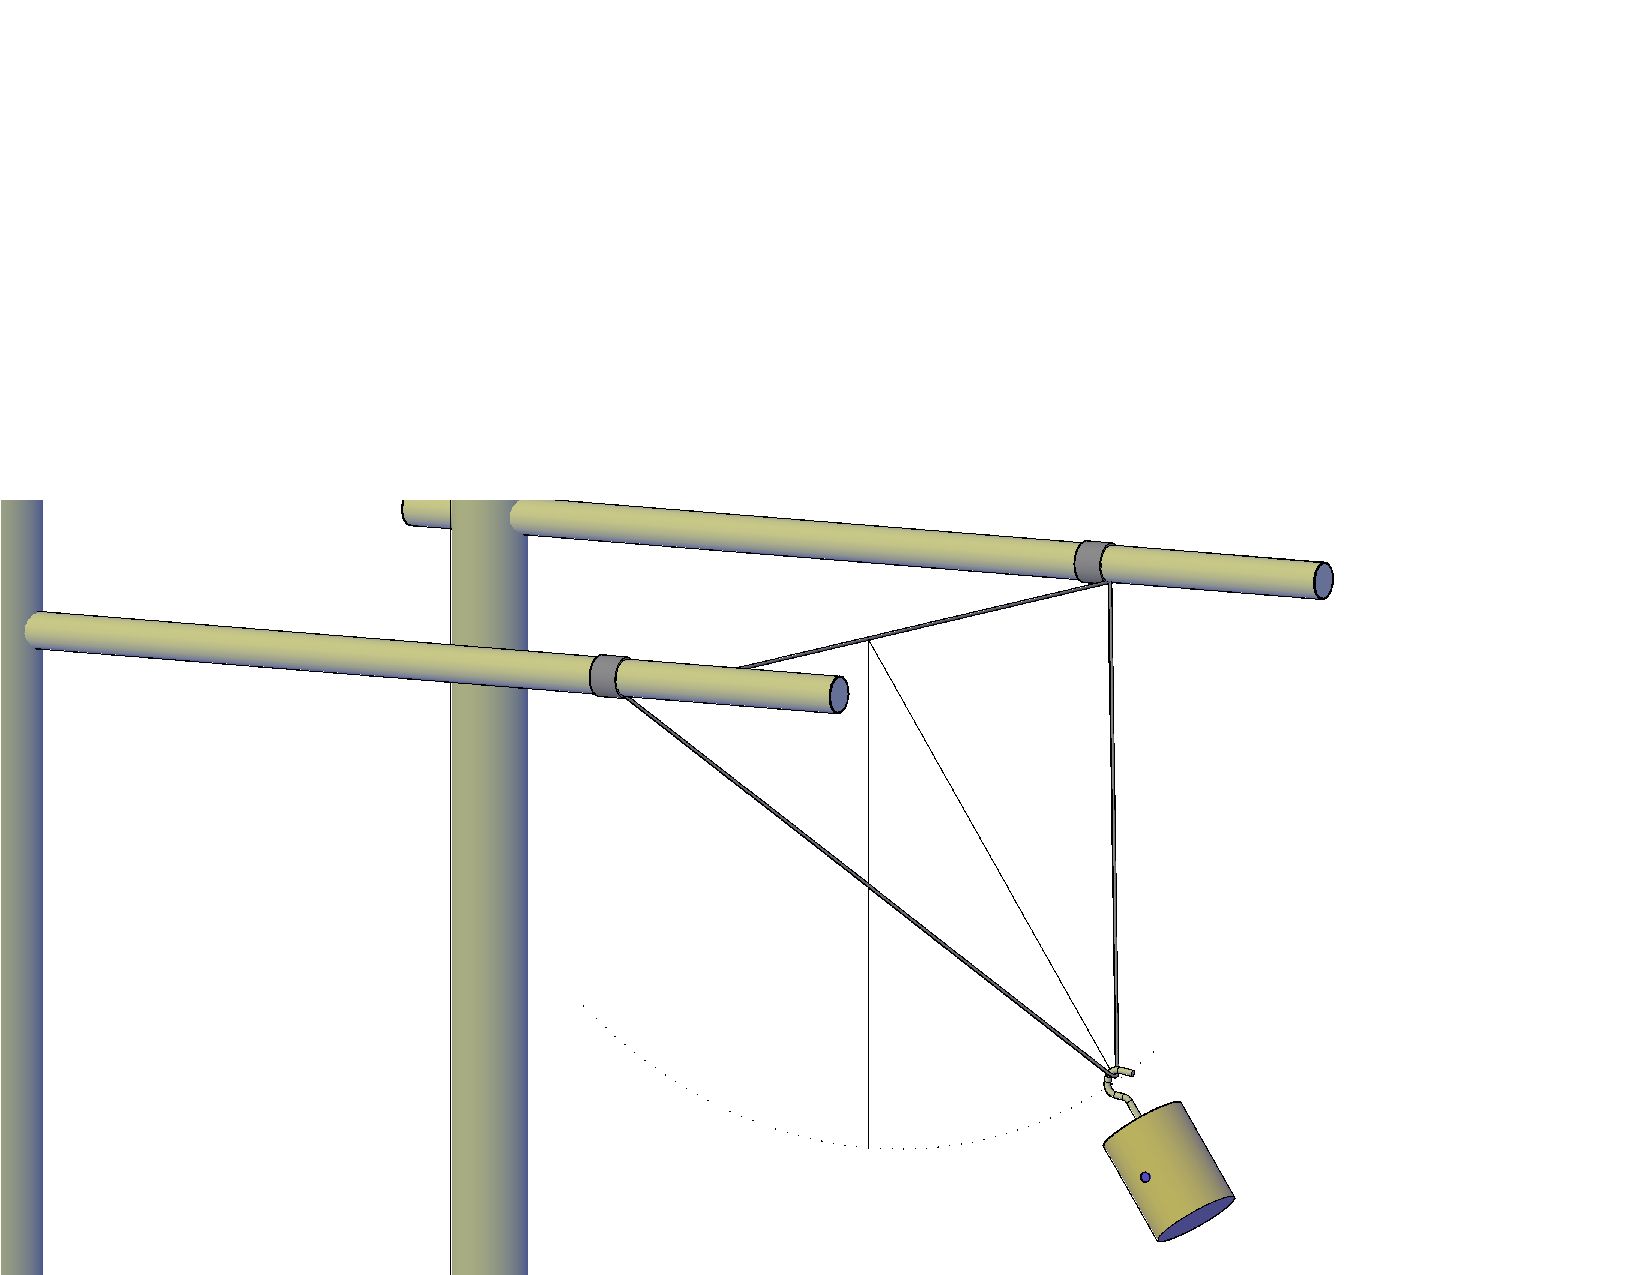
\includegraphics[scale=0.3]{Plots/3dschematic.png}}
\caption{\small{A 3d schematic diagram describing the system used to take all of the data for this report. It is labelled with the relevant variables, as well as a blue dot indicating the object used to optimize the tracking and data recording process.}}
\label{3dschematic}
\end{figure}

The aforementioned sets of data are taken as an MP4 file using an iPhone, and imported to the application 'Tracker: Video Analysis and Modelling Tool'. Tracker uses automated RGB line profiling to record the position of an object at any given time \cite{tracker}. In order to truly exploit the full power and accuracy of this application, distinct variability between the colour of the object being tracked and the colour of the backdrop are essential prerequisites for obtaining clean and accurate results. As such, a piece of blue tape of approximately 5mm diameter is placed on the centre of mass of each weight used. This allows for Tracker to swiftly differentiate between the weight and any other object in the frame of the recording between time steps. With that being said, uncertainty in each recorded value arises due to the size of the tape being used: Tracker simply pinpoints a location that matches the previous RGB reading (up to 20\% evolution), which leaves a 5mm variability between possible recordings. This variability (and resulting implications) is discussed in further detail in the uncertainty analysis section of the report. After recording the position of the weights at each time step, Tracker provides a three dimensional \texttt{.txt} file indicating the $(x, y)$ coordinates of the weight at each time step. All of these files are imported to Python and fitted, using SciPy's \texttt{curve\_fit}, to the functional form of Eq.(\ref{ode small}). The values of $\theta_0$, $T$ and $\tau$ are optimized to replicate the data as accurately as possible, values of which are then used to test the validity of the theoretical claims made in the introduction. \\[0.20cm]
